\documentclass[tikz,border=2pt]{standalone}

\usepackage{pgfplots}

\usepgfplotslibrary{}
\pgfplotsset{compat=1.18,width=4.5cm}


\begin{document}
	
	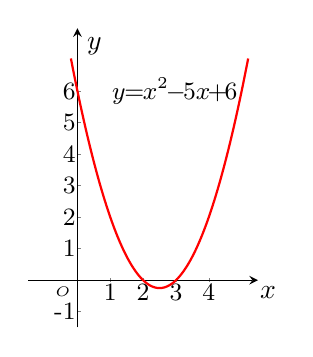
\begin{tikzpicture}
		\begin{axis}
			[,axis lines=center,
			no markers,xmin=-1.5,xmax=5.5,
			ymax=8,ymin=-1.5,		
			xticklabels={1,2,3,4},
			xtick={1,2,3,4},
			xtick distance=1,
			ytick distance=1,
			ytick={-1,1,2,3,4,5,6},
			yticklabels={-1,1,2,3,4,5,6},
			yticklabel style={font=\small\rmfamily},
			xticklabel style={font=\small\rmfamily},
			ytick align=inside,
			y=0.4cm,
			major tick length=0.5mm, 
			,yticklabel shift=-1mm,
			xticklabel shift=-1mm,
			ylabel=$y$,xlabel=$x$,
			xlabel shift=-1em,
			ylabel shift=1cm,
			xlabel style={xshift=1em,yshift=-1em}
			]
			\addplot+ [samples=100,domain=-0.2:5.2,red,thick]{x^2-5*x+6};
			\addplot[samples at={5}]{x^2-5*x+6}node[left=-2pt]{\small $y\!\!=\!\!x^2\!\!-\!\!5x\!\!+\!\!6$};
			\node at(0,0) [below left=-1pt]{\tiny $O$};
		\end{axis}
	\end{tikzpicture}
\end{document}